\documentclass[a4paper,12pt]{article}
\usepackage[T1]{fontenc}
\usepackage[utf8]{inputenc}
\usepackage{amsmath, amssymb, amsthm}
\usepackage{geometry}
\usepackage{xcolor}
\usepackage{titlesec}
\usepackage{enumitem}
\usepackage{booktabs}
\usepackage{array}
\usepackage{hyperref}
\usepackage{setspace}
\usepackage{fancyhdr}
\usepackage{float}
\usepackage{colortbl}
\usepackage{graphicx}

% ---- Margenes ----
\geometry{top=2.2cm, bottom=2.2cm, left=3cm, right=2.5cm}

% ---- Interlineado ----
\setstretch{1.15}

% ---- Colores ----
\definecolor{rojoras}{RGB}{160,35,25}
\definecolor{grisclaro}{RGB}{242,242,242}
\definecolor{verdest}{RGB}{0,110,60}
\definecolor{azulsis}{RGB}{30,90,160}

% ---- Encabezado ----
\pagestyle{fancy}
\fancyhf{}
\lhead{\small\textit{INFORME TÉCNICO: AUTOCORRELACIÓN ESPACIAL}}
\rhead{\small\textit{UNA Puno, 2026}}
\cfoot{\thepage}
\renewcommand{\headrulewidth}{0.4pt}
\setlength{\headheight}{14pt}

% ---- Traducciones manuales ----
\renewcommand{\figurename}{Figura}
\renewcommand{\tablename}{Tabla}
\renewcommand{\refname}{Referencias}

% ---- Formato de secciones ----
\titleformat{\section}{\large\bfseries\color{azulsis}}{}{0em}{}%
  [\vspace{-5pt}\rule{\linewidth}{0.5pt}\vspace{1pt}]
\titleformat{\subsection}{\normalsize\bfseries\itshape}{}{0em}{}
\titlespacing{\section}{0pt}{12pt}{4pt}
\titlespacing{\subsection}{0pt}{7pt}{3pt}

% ---- Hiperlinks ----
\hypersetup{colorlinks=true, linkcolor=azulsis, citecolor=azulsis, urlcolor=azulsis}

% ---- Espaciado de parrafos ----
\setlength{\parskip}{4pt}
\setlength{\parindent}{1.2em}


\begin{document}
\thispagestyle{empty}

\begin{center}

% ===== UNIVERSIDAD =====
{\large \textbf{UNIVERSIDAD NACIONAL DEL ALTIPLANO}}\\[0.2cm]
{\normalsize Facultad de Ingeniería Estadística e Informática}\\
{\normalsize Escuela Profesional de Ingeniería Estadística e Informática}\\[1.5cm]

% ===== LOGO =====
\vspace{1.5cm}
{\Huge\bfseries\color{azulsis} FIEI}\\[0.5cm]
{\large\textit{Facultad de Ingeniería Estadística e Informática}}\\[1.5cm]

% ===== TÍTULO =====
\begin{spacing}{1.2}
{\LARGE \textbf{Diseño e Implementación de un Aplicativo Web para el Análisis y Visualización de Autocorrelación Espacial usando Índices de Moran Global y Local (LISA)}}\\[0.2cm]
\end{spacing}

\vspace{1.5cm}
\rule{12cm}{0.8pt}
\vspace{1.5cm}

% ===== DATOS =====
\begin{tabular}{rl}
\textbf{Autor:}   & Noe Ulises Machaca Chambilla \\[0.3cm]
\textbf{Docente:} & Fred Torres Cruz    \\[0.3cm]
\textbf{Curso:}   & Estadística Espacial    \\[0.3cm]
\end{tabular}

\vfill

% ===== LUGAR Y FECHA =====
{\normalsize Puno -- Perú}\\
{\normalsize Junio, 2026}

\end{center}

\newpage

\section{Introducción}
El análisis espacial es una rama crucial de la ciencia de datos y la estadística aplicada, caracterizada por la modelación de fenómenos donde la localización geográfica de las observaciones desempeña un papel determinante. En la estadística clásica, se suele asumir que las observaciones muestrales son independientes e idénticamente distribuidas (i.i.d.). Sin embargo, en los datos geográficos este supuesto es frecuentemente violado debido a la existencia de la dependencia espacial. 

Como enunció Waldo Tobler en su \textit{Primera Ley de la Geografía}: \textit{"Todo está relacionado con todo lo demás, pero las cosas cercanas están más relacionadas que las cosas lejanas"}. La autocorrelación espacial cuantifica esta ley física, permitiendo evaluar si un determinado atributo medido sobre unidades espaciales (como distritos, estados o parcelas) se distribuye de manera aleatoria, dispersa o agrupada. 

Para facilitar la comprensión, estimación y análisis de este fenómeno, el presente informe detalla el desarrollo e implementación de un aplicativo web interactivo en Python utilizando el framework \textbf{Streamlit}. Esta herramienta procesa múltiples conjuntos de datos espaciales reales y estima de manera dinámica el Índice de Moran Global y los Indicadores Locales de Asociación Espacial (LISA), proporcionando visualizaciones geográficas interactivas modernas que superan las representaciones estáticas tradicionales.

\section{Fundamento Estadístico y Conceptual}

\subsection{La Matriz de Pesos Espaciales (W)}
La formalización matemática de la proximidad espacial se concreta mediante la construcción de la Matriz de Pesos Espaciales ($W$), la cual define la topología de la vecindad. Para un sistema con $N$ regiones, $W$ es una matriz cuadrada de dimensión $N \times N$:
\[
W = \begin{pmatrix}
w_{11} & w_{12} & \cdots & w_{1N} \\
w_{21} & w_{22} & \cdots & w_{2N} \\
\vdots & \vdots & \ddots & \vdots \\
w_{N1} & w_{N2} & \cdots & w_{NN}
\end{pmatrix}
\]
Donde $w_{ij}$ representa la fuerza de la interacción espacial entre la región $i$ y la región $j$. Por convención, la diagonal principal se define como cero ($w_{ii} = 0$) para evitar la auto-influencia.

En este aplicativo se implementan los dos criterios de contigüidad basados en fronteras más utilizados:
\begin{enumerate}
    \item \textbf{Contigüidad Queen (Reina):} Dos regiones $i$ y $j$ se consideran vecinas si comparten al menos un límite común, sea este una frontera lineal (arista) o un solo punto de vértice común. Es el criterio más amplio.
    \item \textbf{Contigüidad Rook (Torre):} Dos regiones se consideran vecinas únicamente si comparten una frontera lineal común (arista). Se descartan las uniones por vértices aislados.
\end{enumerate}

Para corregir el impacto de la cantidad desigual de vecinos de cada región y normalizar el rezago espacial, la matriz $W$ se somete a una estandarización por filas (operador `transform = 'r'` en PySAL):
\[
w_{ij}^{std} = \frac{w_{ij}}{\sum_{j=1}^N w_{ij}}
\]
Esto garantiza que la suma de cada fila de la matriz sea igual a 1, interpretando el rezago espacial como el promedio ponderado de los valores de los vecinos.

\subsection{Índice de Moran Global}
El Índice de Moran Global ($I$) cuantifica el grado general de autocorrelación espacial lineal de una variable continua $x$ sobre todo el territorio. Matemáticamente, se expresa de la siguiente manera:
\[
I = \frac{N}{S_0} \frac{\sum_{i=1}^N \sum_{j=1}^N w_{ij}(x_i - \bar{x})(x_j - \bar{x})}{\sum_{i=1}^N (x_i - \bar{x})^2}
\]
Donde $\bar{x}$ es la media muestral de la variable y $S_0$ es la suma de todos los pesos en la matriz original:
\[
S_0 = \sum_{i=1}^N \sum_{j=1}^N w_{ij}
\]
El valor del índice oscila teóricamente entre $-1$ y $+1$ (aunque los límites reales dependen de la matriz de pesos específica):
\begin{itemize}
    \item \textbf{Autocorrelación Positiva ($I > E(I)$):} Indica que valores similares (altos con altos, o bajos con bajos) tienden a ubicarse cerca en el espacio, formando clústeres.
    \item \textbf{Autocorrelación Negativa ($I < E(I)$):} Indica que regiones vecinas tienden a tener valores muy diferentes, asemejándose a un patrón de tablero de ajedrez (dispersión).
    \item \textbf{Ausencia de Autocorrelación ($I \approx E(I)$):} El patrón espacial del atributo es puramente aleatorio.
\end{itemize}

Para la inferencia estadística, la significancia del índice obtenido se evalúa bajo la hipótesis nula de aleatoriedad espacial completa. Esto se realiza mediante el cálculo de un Z-score y su correspondiente p-valor, utilizando simulaciones de Monte Carlo con permutaciones aleatorias (usualmente 999 permutaciones en la librería `esda`):
\[
Z_I = \frac{I - E(I)}{\sqrt{Var(I)}}
\]

\subsection{Índice de Moran Local (LISA)}
El Índice de Moran Global proporciona una medida sintética general, pero puede enmascarar la heterogeneidad espacial (la existencia de patrones diferenciados en diferentes subregiones). Luc Anselin (1995) propuso los Indicadores Locales de Asociación Espacial (LISA). El Moran Local ($I_i$) mide el aporte individual de cada unidad espacial $i$ al patrón global:
\[
I_i = \frac{x_i - \bar{x}}{m_2} \sum_{j=1}^N w_{ij}(x_j - \bar{x})
\]
Donde:
\[
m_2 = \frac{\sum_{i=1}^N (x_i - \bar{x})^2}{N}
\]
El análisis LISA permite clasificar a las regiones estadísticamente significativas ($p < 0.05$) en cuatro cuadrantes de asociación espacial, según el valor estandarizado de la región y el de su rezago:
\begin{itemize}
    \item \textbf{High-High (HH) [Cuadrante I]:} Valor alto rodeado de valores promedio altos. Se les conoce como clústeres calientes (\textit{hotspots}). Coloreados de rojo.
    \item \textbf{Low-High (LH) [Cuadrante II]:} Valor bajo rodeado de valores altos. Constituye una anomalía espacial (\textit{outlier}). Coloreados de celeste.
    \item \textbf{Low-Low (LL) [Cuadrante III]:} Valor bajo rodeado de valores promedio bajos. Se les conoce como clústeres fríos (\textit{coldspots}). Coloreados de azul.
    \item \textbf{High-Low (HL) [Cuadrante IV]:} Valor alto rodeado de valores bajos. Constituye una anomalía espacial (\textit{outlier}). Coloreados de rojo claro.
\end{itemize}

\newpage

\section{Descripción de los Datasets Integrados}

La aplicación incorpora 6 conjuntos de datos clásicos e históricos de la literatura espacial en Python (PySAL), ofreciendo una amplia gama de escenarios de estudio:

\begin{enumerate}
    \item \textbf{Columbus Crime:} Contiene datos de delincuencia residencial, ingresos y valores de las viviendas para 49 vecindarios en Columbus, Ohio, recopilados originalmente por Anselin (1988). Permite evaluar el agrupamiento de los delitos urbanos.
    \item \textbf{Guerry Moral Statistics:} Basado en los datos históricos recopilados por el estadístico André-Michel Guerry en 1833 para 85 departamentos franceses. Incluye variables sobre educación (alfabetización), criminalidad moral, suicidios y donaciones, ideal para analizar la geografía social histórica.
    \item \textbf{US Income:} Serie temporal de ingresos personales per cápita en los 48 estados contiguos de EE.UU. desde 1929 hasta 2009. Para su visualización, la aplicación realiza un acoplamiento (\textit{merge}) espacial en caliente con las geometrías de los estados y permite evaluar la evolución de la disparidad regional de la riqueza.
    \item \textbf{SIDS North Carolina:} Datos sobre la tasa del Síndrome de Muerte Súbita del Lactante (SIDS) en los 100 condados de Carolina del Norte para el período 1974-1984. Es un conjunto de datos clásico de epidemiología para buscar agrupamientos anómalos de mortalidad infantil.
    \item \textbf{Mexico Demographics:} Producto Interno Bruto (PIB) per cápita y variables demográficas de los 32 estados de la República Mexicana desde 1940 hasta 2000. Excelente para evaluar la persistencia de la polarización económica norte-sur.
    \item \textbf{Boston Housing:} Datos censales de 506 distritos de la zona metropolitana de Boston recopilados por Harrison y Rubinfeld (1978). Aborda valores inmobiliarios (`MEDV`) y variables de polución por óxidos de nitrógeno (`NOX`), relacionando factores socioeconómicos y ambientales.
\end{enumerate}

\section{Arquitectura Tecnológica del Aplicativo}
La arquitectura de la aplicación sigue una estructura de flujo de datos unidereccional optimizada para la interacción web ágil en Python:

\begin{figure}[H]
    \centering
    \begin{tabular}{c}
        \textbf{Arquitectura de Datos del Aplicativo} \\
        \hline
        $\text{[Carga de Datos (GeoPandas / Carga URL)]} \longrightarrow \text{[Cálculo de Pesos (libpysal)]}$ \\
        $\downarrow$ \\
        $\text{[Inferencia Global (Moran)]} \longleftrightarrow \text{[Inferencia Local (LISA)]}$ \\
        $\downarrow$ \\
        $\text{[Renderizado en UI: Streamlit (Folium / Plotly Express)]}$
    \end{tabular}
    \caption{Flujo lógico de procesamiento geoestadístico en la aplicación.}
\end{figure}

El uso de `streamlit.components.v1.html` permite renderizar los mapas interactivos de Folium de forma estática en iFrames, impidiendo que el motor de Streamlit reinicie la aplicación entera cuando el usuario realiza un paneo o zoom sobre los mapas.

\newpage

\section{Análisis de la Interfaz y Explicación de Pantallas}

La interfaz ha sido diseñada para guiar de forma didáctica al analista a través de las fases del análisis geoespacial:

\subsection{Ficha Informativa y Selección de Datos}
La barra lateral permite al usuario elegir la fuente de datos (integrados o GeoJSON externo) y seleccionar las variables. Al cambiar de dataset, la aplicación genera un cuadro informativo que describe la variable seleccionada y proporciona contexto educativo inmediato (Figura \ref{fig:sidebar_context}).

\begin{figure}[H]
    \centering
    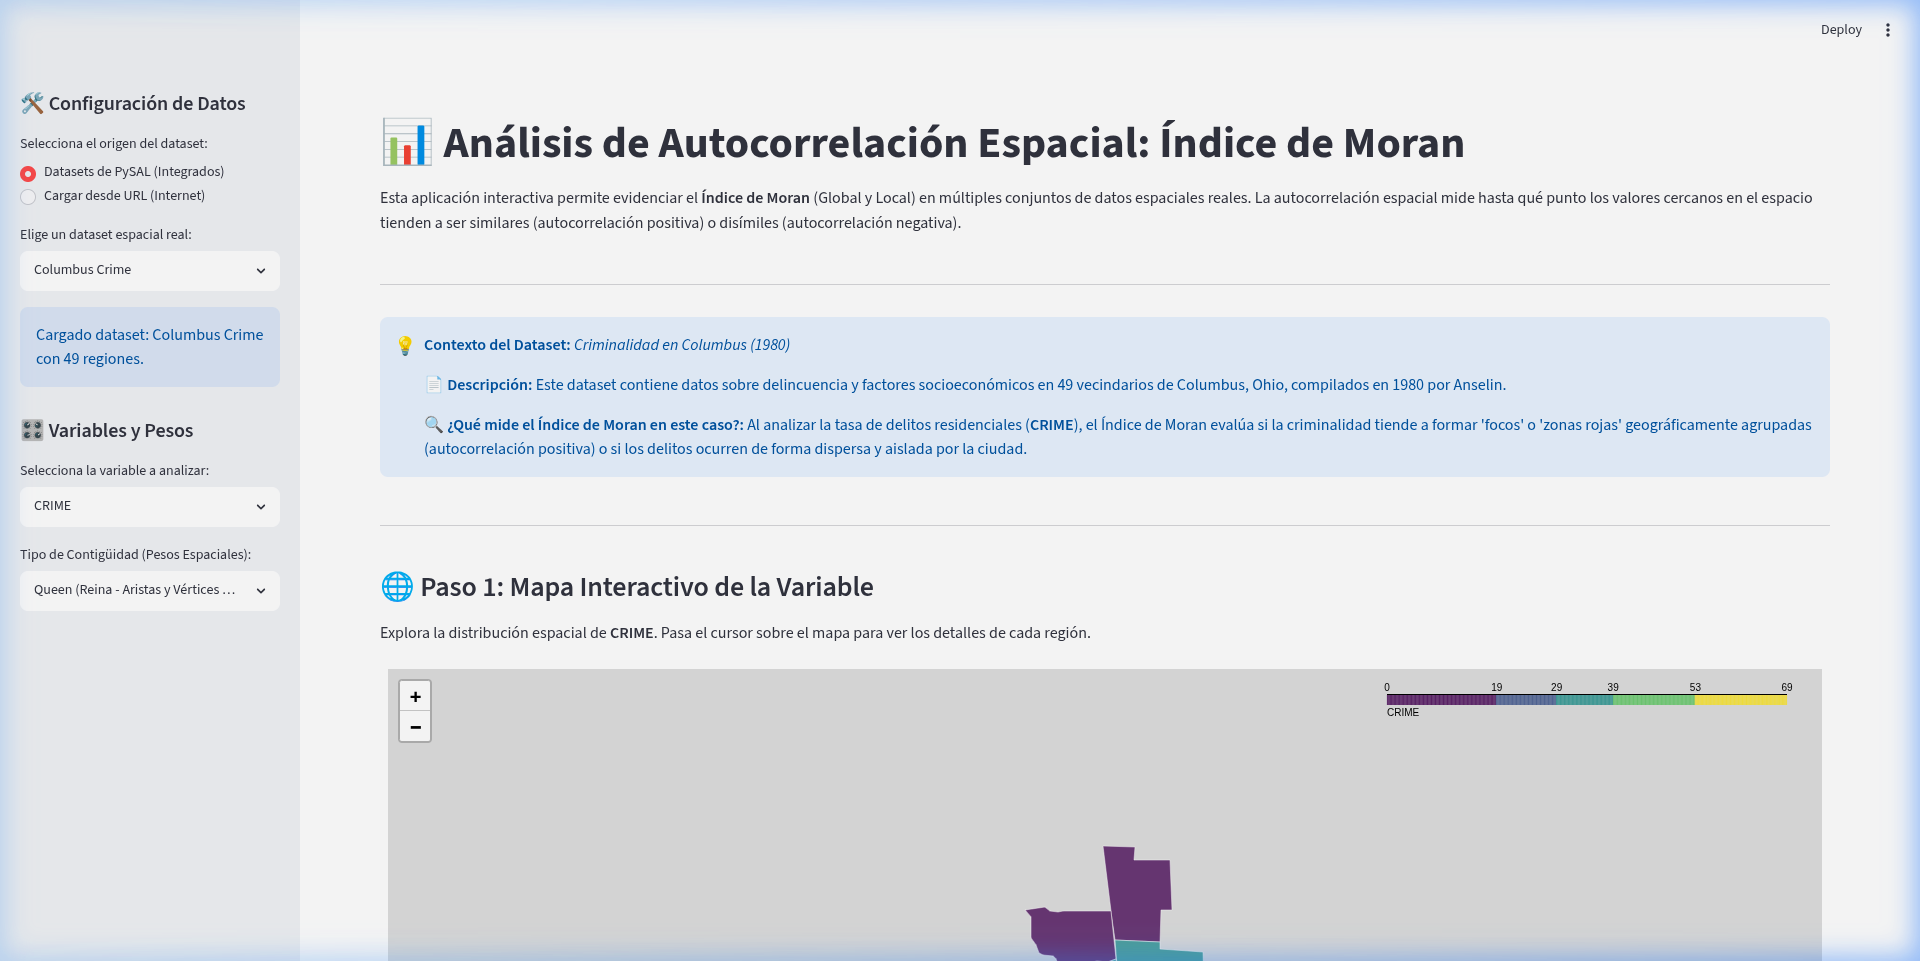
\includegraphics[width=1.0\textwidth]{images/contexto_dataset.png}
    \caption{Barra lateral de configuración de datos y cuadro de contexto educativo dinámico del dataset Columbus Crime.}
    \label{fig:sidebar_context}
\end{figure}

\subsection{Paso 1: Distribución Espacial de la Variable}
Se muestra un mapa interactivo coroplético de la variable original mediante el método `explore` de GeoPandas. La Figura \ref{fig:mapa_original} ilustra la distribución de la tasa de crímenes residenciales en Columbus, Ohio.

\begin{figure}[H]
    \centering
    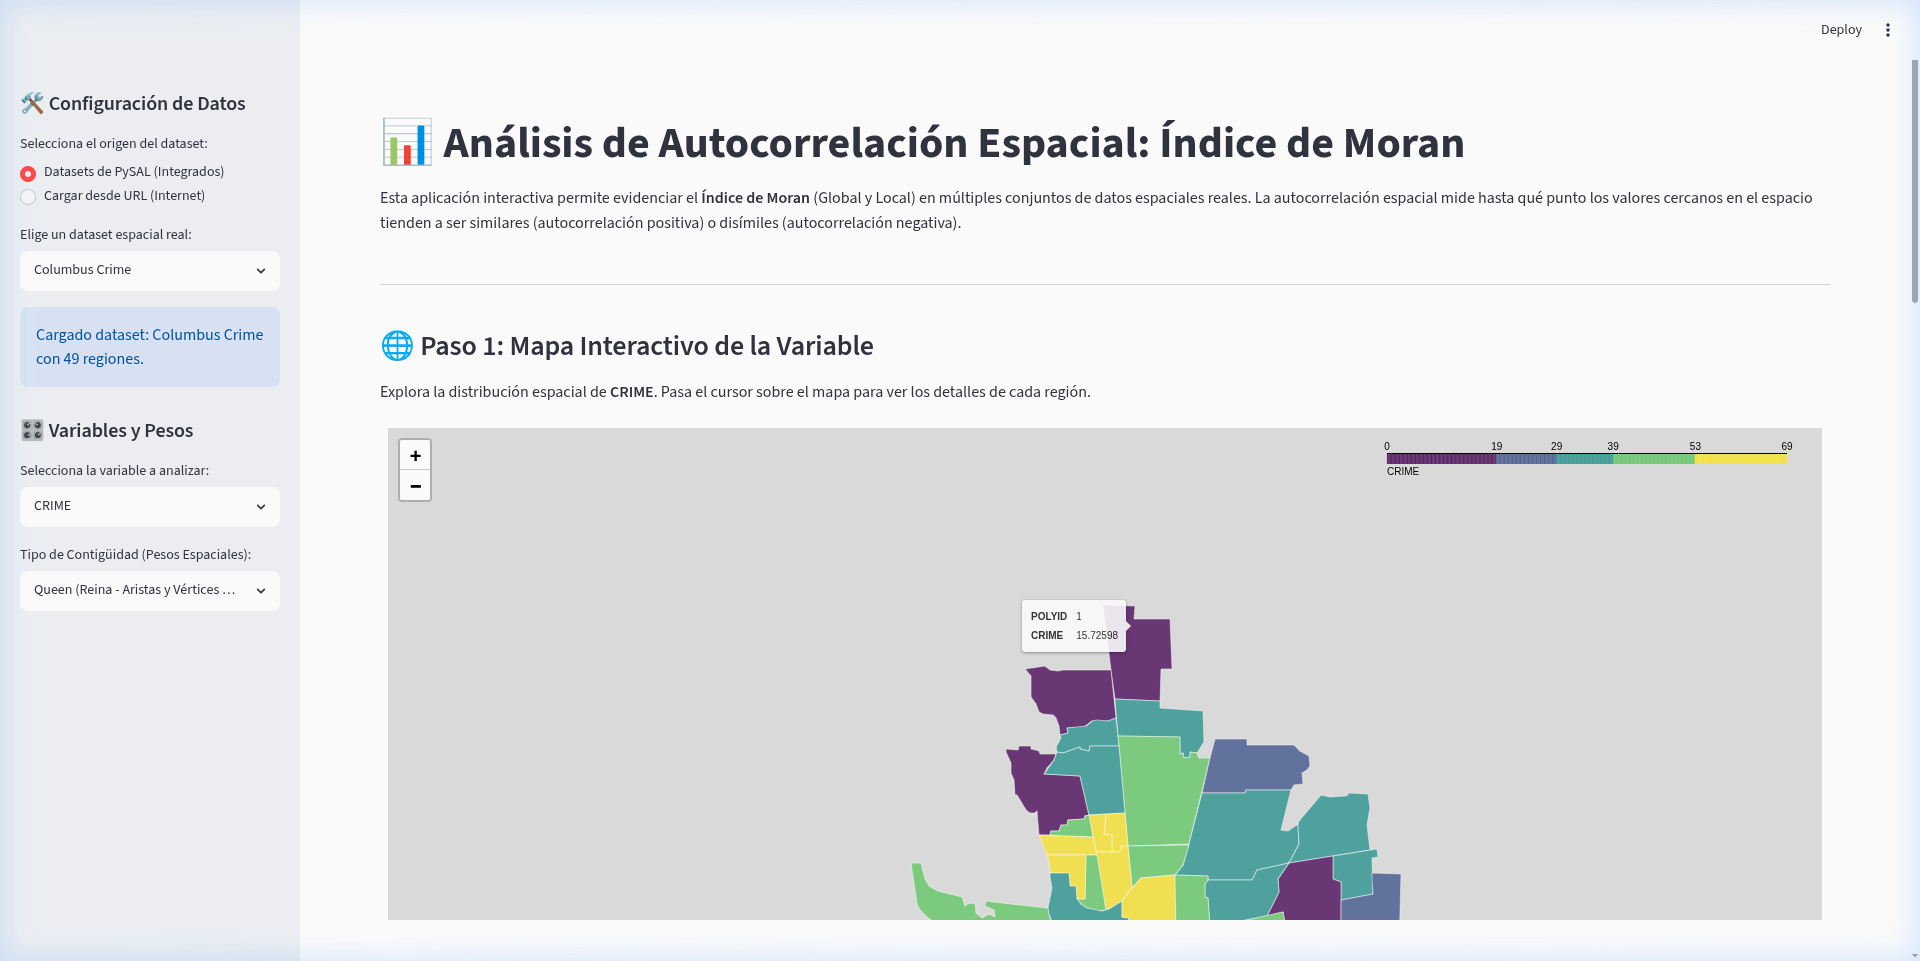
\includegraphics[width=0.95\textwidth]{images/mapa_interactivo.png}
    \caption{Mapa interactivo de la variable original (delitos) con tooltip activo en el vecindario 1.}
    \label{fig:mapa_original}
\end{figure}

\subsection{Paso 2: Moran Scatterplot e Inferencia Global}
El aplicativo calcula el Índice de Moran Global y visualiza las métricas críticas ($I$, P-Valor y Z-Score) junto con un texto de interpretación automatizado. Adicionalmente, dibuja un \textit{Moran Scatterplot} dinámico en Plotly, donde la pendiente de la recta de regresión ajustada representa exactamente el valor del Índice de Moran Global (Figura \ref{fig:step2}).

\begin{figure}[H]
    \centering
    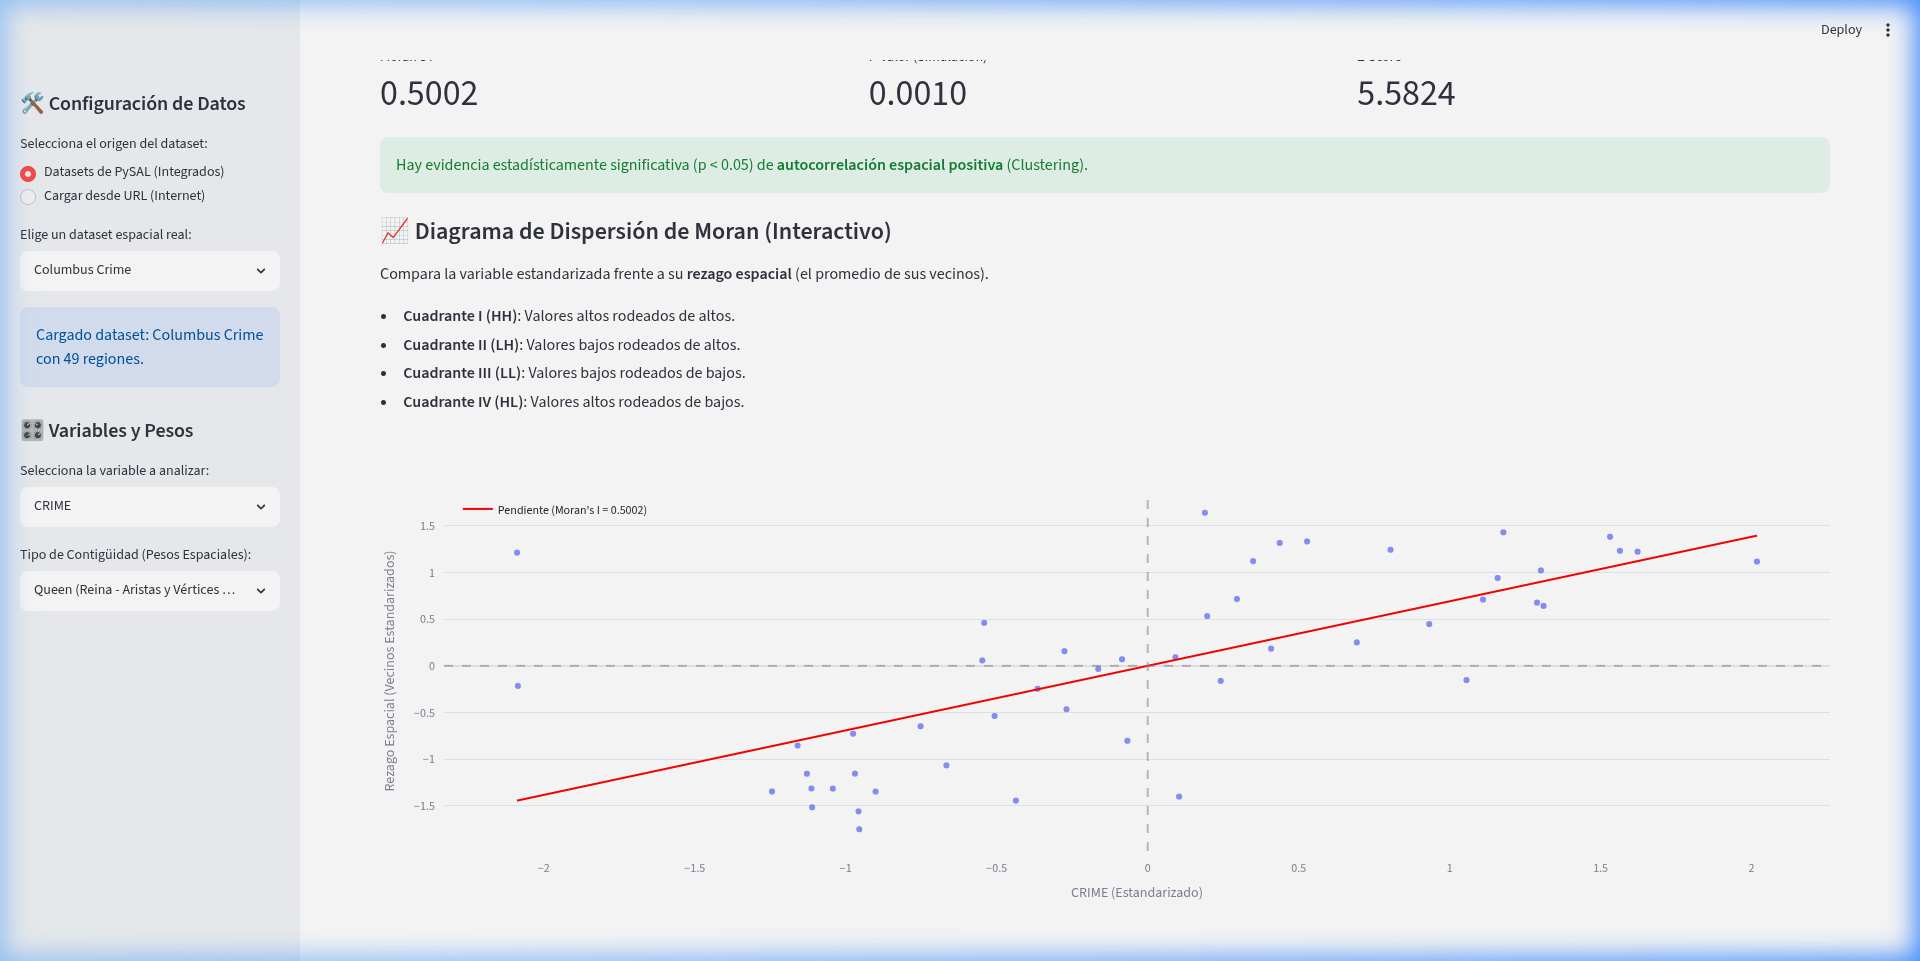
\includegraphics[width=0.95\textwidth]{images/step2_scatterplot.png}
    \caption{Métricas del Índice de Moran Global e interpretación y Diagrama de Dispersión interactivo de Moran.}
    \label{fig:step2}
\end{figure}

\subsection{Paso 3: Análisis de Clústeres Locales (LISA)}
El mapa interactivo del Índice de Moran Local clasifica geográficamente las áreas según sus agrupamientos estadísticamente significativos (Figura \ref{fig:step3}).

\begin{figure}[H]
    \centering
    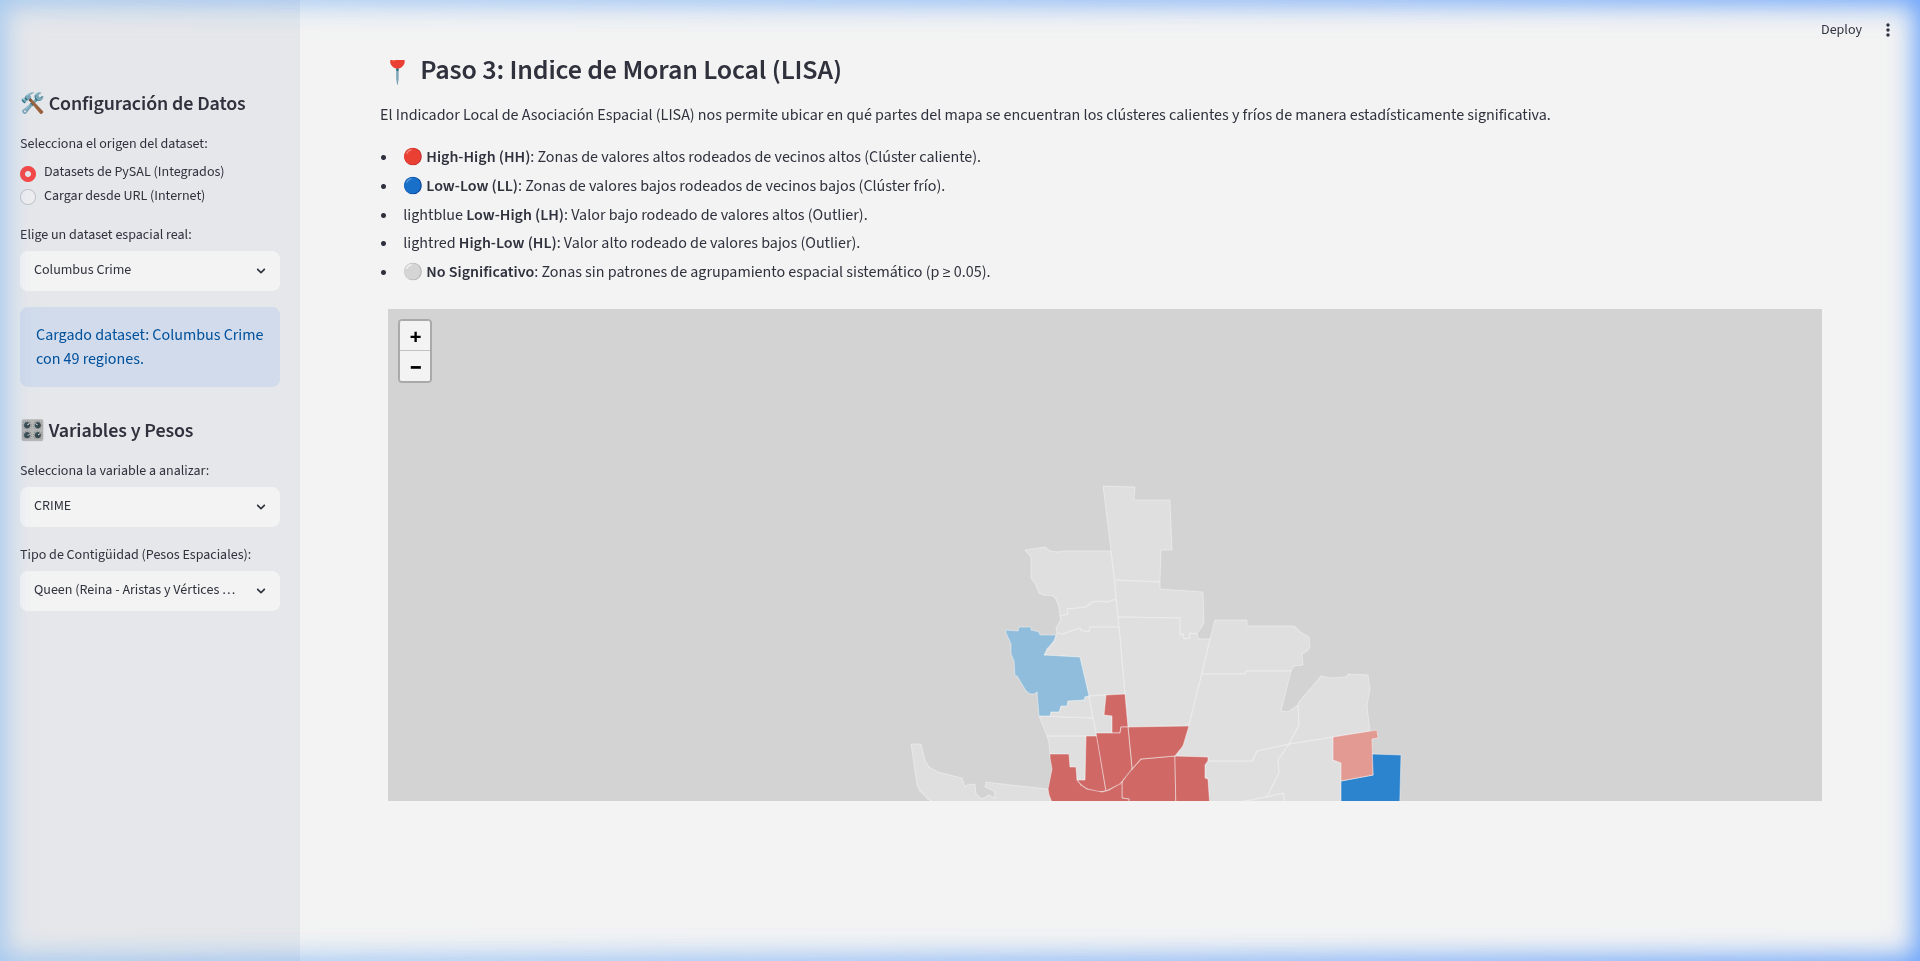
\includegraphics[width=0.95\textwidth]{images/step3_lisa.png}
    \caption{Mapa de Clústeres LISA para Columbus Crime, donde se observan clústeres calientes en rojo (centro-norte) y fríos en azul (sur).}
    \label{fig:step3}
\end{figure}

\newpage

\subsection{Demostración Multi-Dataset: SIDS North Carolina}
Para evidenciar la flexibilidad del aplicativo, al seleccionar el dataset de SIDS (Síndrome de Muerte Súbita del Lactante en Carolina del Norte), la aplicación calcula automáticamente las nuevas matrices de contigüidad para los 100 condados. La Figura \ref{fig:sids2} muestra el diagrama de dispersión para la tasa de SIDS en 1979 ($I = 0.1431$, indicando autocorrelación espacial positiva moderada), mientras que la Figura \ref{fig:sids3} revela los condados calientes concentrados en el noreste y los fríos en el oeste del estado.

\begin{figure}[H]
    \centering
    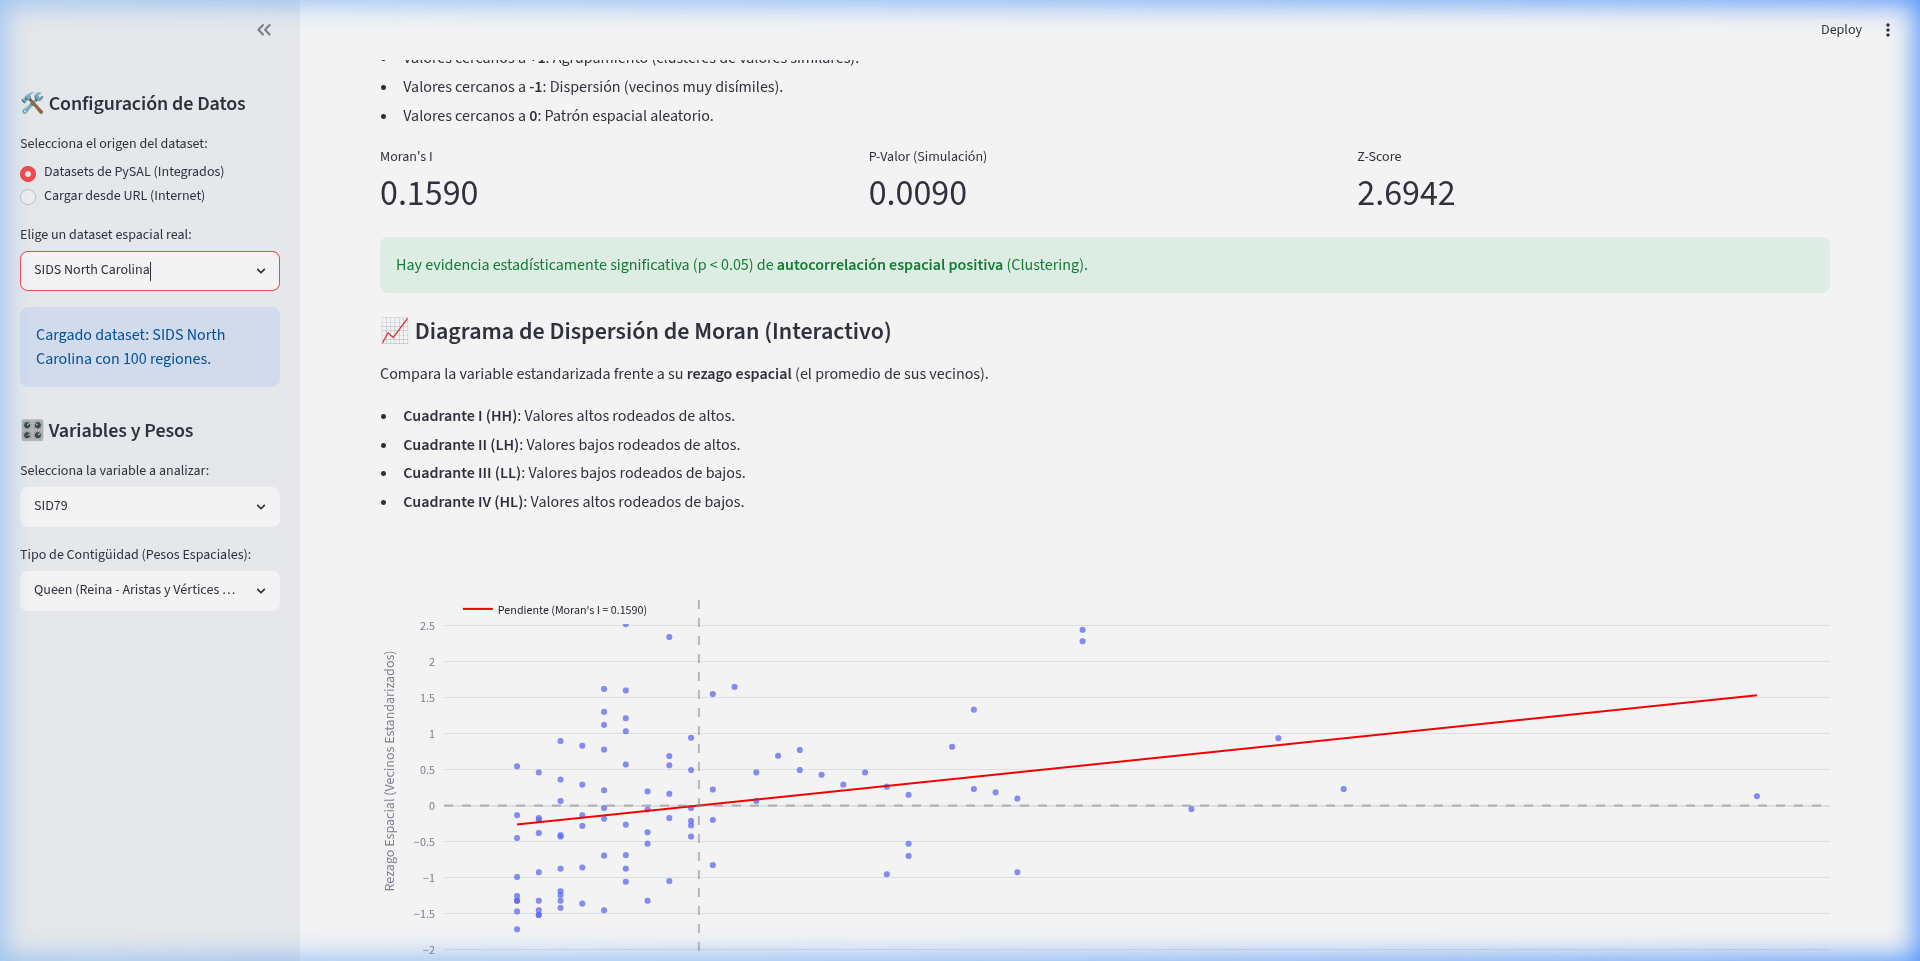
\includegraphics[width=0.9\textwidth]{images/sids_step2.png}
    \caption{Métricas y Diagrama de Dispersión de Moran para la tasa de SIDS (1979) en Carolina del Norte.}
    \label{fig:sids2}
\end{figure}

\begin{figure}[H]
    \centering
    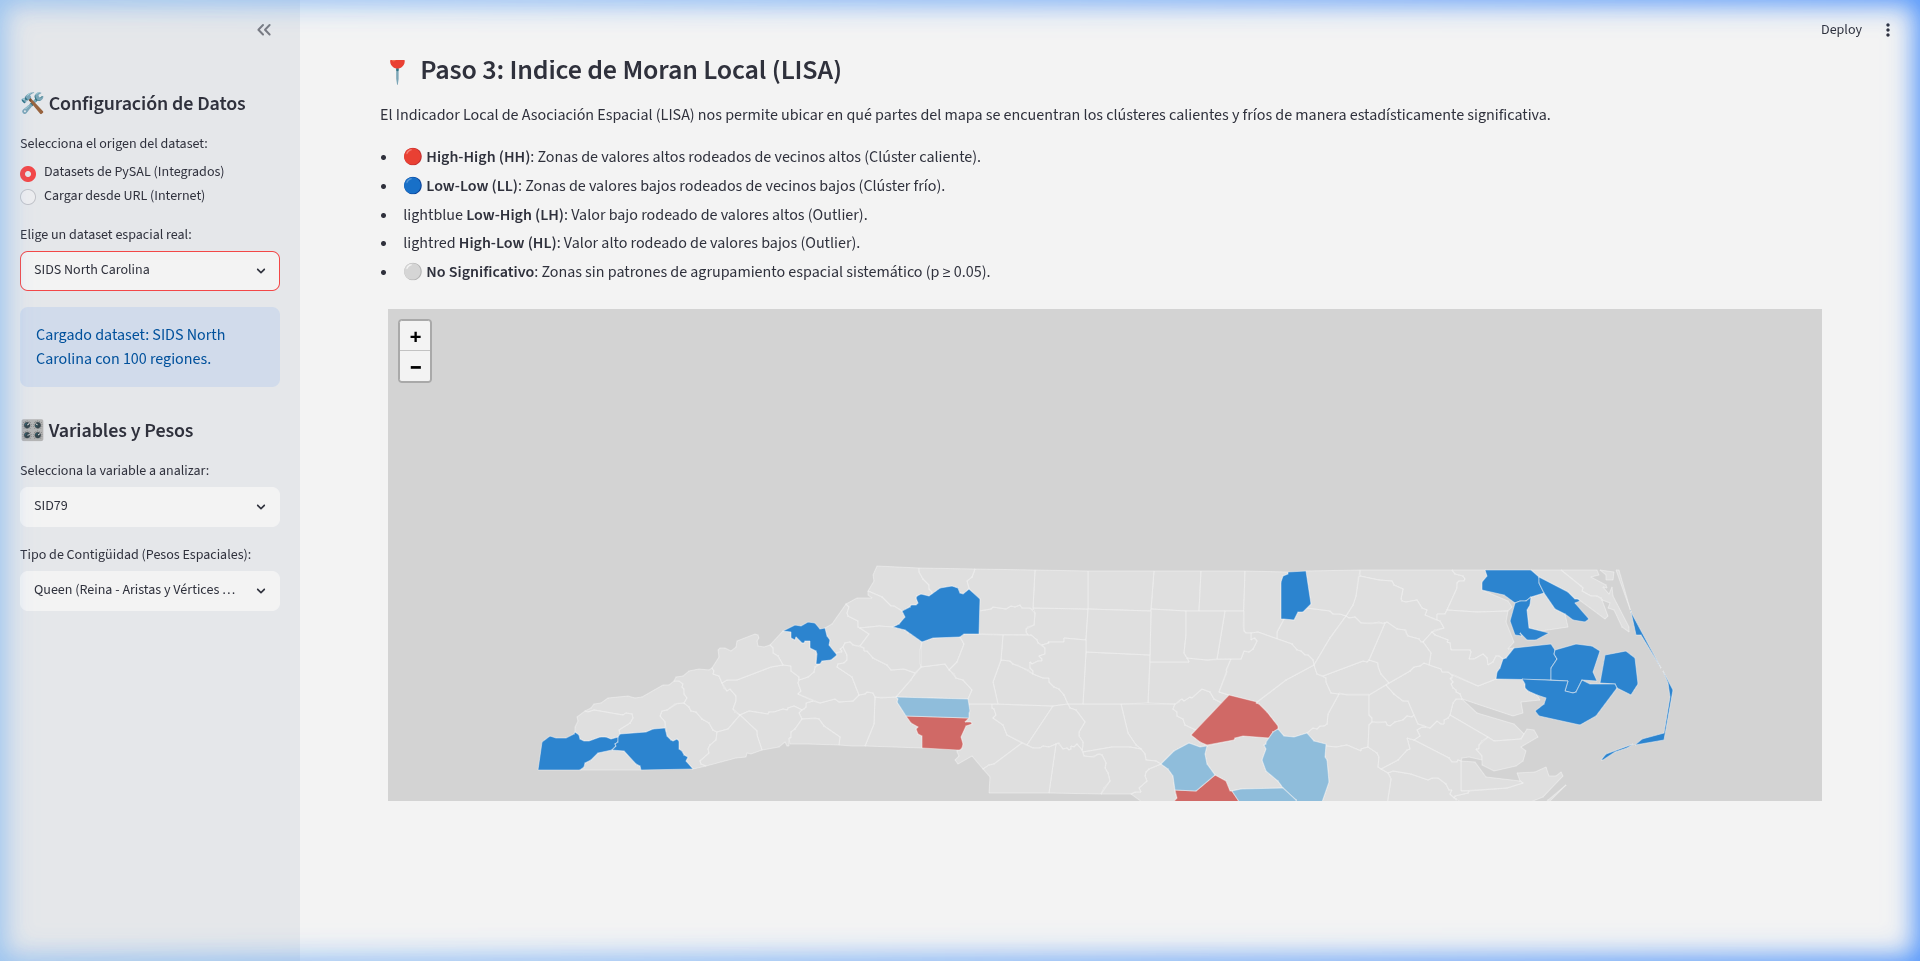
\includegraphics[width=0.9\textwidth]{images/sids_step3.png}
    \caption{Mapa de Clústeres LISA que identifica clústeres calientes y fríos de muerte súbita infantil.}
    \label{fig:sids3}
\end{figure}

\section{Conclusión y Enlace de Despliegue}
El aplicativo interactivo implementado logra traducir complejos conceptos matemáticos de la estadística espacial en visualizaciones dinámicas de fácil interpretación. Permite evaluar de manera directa el impacto de la matriz de contigüidad (Queen vs Rook) en los resultados del Índice de Moran y localizar agrupamientos calientes o anomalías territoriales de interés científico.

La aplicación ha sido configurada y está lista para producción. Su prototipo en la nube puede ejecutarse en el siguiente enlace de despliegue:

\begin{center}
    \url{https://moran-index-app.streamlit.app/}
\end{center}

\end{document}
